\documentclass[10pt]{article}

\newtheorem{mydef}{Определение}
\usepackage{mathtools}
\usepackage{cmap} % for serchable pdf's
\usepackage[utf8]{inputenc}
\usepackage[russian]{babel}
\usepackage{fontspec}
\usepackage{enumerate}
\setmainfont[Mapping=tex-text]{CMU Serif}



\begin{document}
\title{Синтаксический анализ графов и задача генерации строк с ограничениями}
\author{Рустам Азимов, Семён Григорьев \\ 
Санкт-Петербургский государственный университет, \\
Россия, 199034, Санкт-Петербург, Университетская наб. 7/9/ \\ 
\mail{rustam.azimov19021995@gmail.com}, \mail{Semen.Grigorev@jetbrains.com}
}

\maketitle

\begin{abstract}
Одной из задач, изучаемых в теории формальных языков и автоматов, является задача генерации строк, удовлетворяющих заданной системе правил. С другой стороны, существует задача синтаксического анализа графов, то есть поиска определенных путей в графе, метки на ребрах которых образуют строку, принадлежащую заданному формальному языку. В данной работе будет показана связь между этими двумя задачами.

\vspace{1em}
\textbf{Ключевые слова:} синтаксический анализ графов, генерация строк, формальные языки, конъюнктивные грамматики.

\end{abstract}

\section*{Введение}

В таких областях, как графовые базы данных~\cite{azimov-spbu-graphDB}, биоинформатика~\cite{azimov-spbu-Anderson} и др., возникают задачи поиска путей в графах, удовлетворяющих определенным условиям. Например, на искомые пути могут быть наложены ограничения на длину, или производится поиск лишь простых путей. Но при работе со сложными системами зачастую таких ограничений бывает недостаточно. Поэтому широко распространено использование ограничений на метки ребер/вершин путей помеченного графа. В качестве таких ограничений естественно выбрать формальный язык $L$. Тогда при заданном алфавите $\Sigma$ и ориентированном графе $G$, ребра которого помечены символами из $\Sigma$, для искомых путей $p$ графа $G$ выполняется $l(p) \in L$, где $l(p)$ означает слово из $\Sigma^*$, полученное последовательной конкатенацией меток пути $p$. Задачи поиска путей в графе, которые используют такие ограничения с формальными языками, являются задачами синтаксического анализа графов.

Кроме того, существует задача генерации строк, суть которой в построении строк, принадлежащих некоторому формальному языку. В работе~\cite{azimov-spbu-Okhotin} получены оценки сложности задачи генерации строк с дополнительными ограничениями для различных классов формальных языков.

Некоторые вариации задач синтаксического анализа графов могут быть сведены к задаче генерации строк. Так, например, в большинстве задач синтаксического анализа графов требуется найти путь в графе, соответствующий строке некоторого формального языка $L$. Так как все пути в графе соответствуют строкам из некоторого регулярного языка $R$, то в данной задаче требуется найти путь, соответствующий строке из языка $L \cap R$. Эта задача может быть решена с помощью генератора строк рассматриваемого пересечения языков.

Таким образом, в данной работе исследуется связь задачи генерации строк и некоторых типов задач синтаксического анализа графов. В качестве формальных языков будут рассматриваться широко используемые в области синтаксического анализа графов контекстно-свободные языки. Также будут рассмотрены конъюнктивные~\cite{azimov-spbu-conjunctiveGrammar} языки, обладающие большей выразительной мощностью.

\section{Синтаксический анализ графов}
В данном разделе будут даны основные определения из области синтаксического анализа графов, и рассмотрены различные формулировки задач этой области с использованием контекстно-свободных грамматик.

В данной работе пустую строку будем обозначать $\varepsilon$, а конкатенацию двух строк $S_{1}$ и $S_{2}$~--- $S_{1} \cdot S_{2}$.

\begin{mydef}
Граф --- это тройка $G = (Q,\Sigma,\delta)$, где $Q \cap \Sigma =  \emptyset$, $Q$~--- конечное множество вершин графа, $\Sigma$~--- конечный алфавит символов, используемых в качестве меток на ребрах графа, и $\delta \subseteq Q \times \Sigma \times Q$~--- конечное множество ребер, помеченных символами из $\Sigma$.
\end{mydef}
Если $m \in Q$ и $\sigma \in \Sigma$, тогда $\delta(m,\sigma) = \{n~|~(m, \sigma, n) \in \delta\}$ обозначает множество вершин графа, которые имеют входящее ребро из вершины $m$, помеченное символом $\sigma$. Если $m \in Q$ и $S \in \Sigma^*$, то


\[ \delta^*(m, S) =
  \begin{cases}
    \{m\}       & \quad \text{if } S = \varepsilon ;\\
    \cup_{n \in \delta(m, \sigma)} \delta^*(n, S')  & \quad \text{if } S = \sigma \cdot S'.\\
  \end{cases}
\]

Язык, который порождается графом $G$ и выделенными в нем вершинами $m, n \in Q$, обозначим $L(G, m, n)$, где
\[ L(G, m, n) = \{S \in \Sigma^*~|~n \in \delta^*(m, S)\}.
\]

В дальнейшем будут рассматриваться контекстно-свободные грамматики, которые находятся в нормальной форме Хомского~\cite{azimov-spbu-binChomsk}, и в которых исключается вывод пустой строки. Для простоты представления введем следующее определение.

\begin{mydef}
Контекстно-свободная грамматика --- это тройка $C = (N,\Sigma,P)$, где $N \cap \Sigma =  \emptyset$, $N$ --- конечное множество нетерминалов грамматики, $\Sigma$ --- конечный алфавит символов, $P$ --- множество правил грамматики. Кроме того, все правила грамматики записываются в одной из следующих форм: $a \rightarrow b~c$ или $a \rightarrow \sigma$, где $a,b,c \in N$ и $\sigma \in \Sigma$.
\end{mydef}

В данном определении не указывается стартовый нетерминал грамматики, поэтому для определения языка, порождаемого данной грамматикой, необходимо указать соответствующий нетерминал. Тогда язык, порождаемый грамматикой $C$, со стартовым нетерминалом $a \in N$ обозначим $L(C,a)$.

В контексте задач синтаксического анализа графов бывает необходимо отвечать на различного рода вопросы, связанные с искомыми в графе путями. Тип вопросов, на которые отвечает задача принято называть \textit{семантикой запроса}. Далее сформулируем задачи синтаксического анализа графов с использованием КС-грамматики $C$ и различных семантик запросов, рассмотренных в работах~\cite{azimov-spbu-hellings1, azimov-spbu-hellings2}.

Использование \textit{relational} семантики запроса означает, что для нетерминала $a \in N$ и графа $G$ необходимо построить множество $\{(m, n)~|~L(C,a) \cap L(G,m,n) \neq \emptyset \}$.

Использование \textit{all-path} семантики запроса означает, что для нетерминала $a \in N$, графа $G$ и его вершин $m,n \in Q$, необходимо предъявить все пути из вершины $m$ в вершину $n$, такие что метки на ребрах этих путей образуют строку из языка $L(C,a)$.

Использование \textit{single-path} семантики запроса означает, что для нетерминала $a \in N$, графа $G$ и его вершин $m,n \in Q$, необходимо предъявить какой-нибудь путь (если он существует) из вершины $m$ в вершину $n$, такой что метки на ребрах этого пути образуют строку из языка $L(C,a)$.

В качестве грамматики, порождающей язык $L(C,a) \cap L(G,m,n)$, в работе~\cite{azimov-spbu-hellings2} используется \textit{аннотированная грамматика}, определенная следующим образом.

\begin{mydef}
Пусть имеется КС-грамматика $C = (N,\Sigma,P)$ и граф $G = (Q,\Sigma,\delta)$. Тройки $(a,m,n) \in N \times Q \times Q$ будем обозначать $a[m,n]$. Тогда аннотированная грамматика --- это КС-грамматика $C_{G} = (N_{G}, \Sigma, P_{G})$, в которой $N_{G} \subseteq N \times Q \times Q$; каждое правило из $P_{G}$ вида $a[m,n] \rightarrow b[m,o]~c[o,n]$ или вида $a[m,n] \rightarrow \sigma$, где $a,b,c \in N$, $m, n, o \in Q$ и $\sigma \in \Sigma$; и выполняются следующие три правила:

\begin{enumerate}
\item $a[m,n] \in N_{G} \Leftrightarrow L(C,a) \cap L(G,m,n) \neq \emptyset$,
\item $(a[m,n] \rightarrow b[m,o]~c[o,n]) \in P_{G} \Leftrightarrow (a \rightarrow b~c) \in P$,
\item $(a[m,n] \rightarrow \sigma) \in P_{G} \Leftrightarrow (m, \sigma, n) \in \delta \wedge (a \rightarrow \sigma) \in P$.
\end{enumerate}

\end{mydef}

\section{Конъюнктивные грамматики}
В работе будут рассматриваться конъюнктивные грамматики~\cite{azimov-spbu-conjunctiveGrammar}, которые представляют собой расширение контекстно-свободных грамматик операцией пересечения.

\begin{mydef}
Конъюнктивная грамматика~--- это четверка $C =$ \\ $(\Sigma, N, P, S)$, где $N \cap \Sigma =  \emptyset$, $N$~--- конечное множество нетерминалов грамматики, $\Sigma$~--- конечный алфавит символов, $P$~--- множество правил грамматики, а $S$~--- стартовый нетерминал. Кроме того, все правила грамматики имеют вид $a \rightarrow \alpha_{1}~\& \ldots \&~\alpha_{n}$, где $a \in N$, $\alpha_{i} \in (\Sigma \cup N)^*$, $n \ge 1$.
\end{mydef}

Язык, порождаемый конъюнктивной грамматикой, определяется с помощью вывода, в котором на каждом шаге выполняется одно из двух действий:
\begin{itemize}
    \item нетерминал заменяется телом правила, заключенным в скобки;
    \item подстрока вида $(w~\& \ldots \&~w)$, где $w \in \Sigma^*$, заменяется одной строкой $w$.
\end{itemize}

\section{Сложность задачи генерации строк}
В данном разделе будут рассмотрены формулировки задачи генерации строк, приведенные в работе~\cite{azimov-spbu-Okhotin}, и оценки сложности этих задач.

Далее рассмотрим формулировки задачи генерации строк, приведенные в работе~\cite{azimov-spbu-Okhotin}. В данной работе генерируемую строку ограничивают с одной или с двух сторон либо длиной, либо лексикографическим отношением ($\preceq, \succeq$) с другой строкой. Всего приведены пять формулировок задачи генерации строк, использующие такого рода ограничения. Эти задачи и сводимости между ними приведены на рис.~\ref{azimov-spbu-tasks}.

\begin{figure}[h!]
 \centering
 \includegraphics[width=5cm]{pictures/azimov-spbu-okhotin_pic1.png}
 \caption{Сводимости между различными формулировками задачи (взято из работы~\cite{azimov-spbu-Okhotin})}
 \label{azimov-spbu-tasks}
\end{figure}

Из-за существования такого рода сходимостей все пять задач имеют одинаковую сложность для рассмотренных в работе~\cite{azimov-spbu-Okhotin} классов грамматик, среди которых имеются классы контекстно-свободных и конъюнктивных грамматик. В таблице~\ref{azimov-spbu-table} приведена сложность задач принадлежности, пустоты и генерации строк с ограничениями для классов $CF$ --- контекстно-свободных и $Conj$ --- конъюнктивных грамматик.

\begin{table}[h!]
 \centering
  \caption{Сложность задач для грамматик, подразумевается полнота
для указанных классов (фрагмент таблицы из работы~\cite{azimov-spbu-Okhotin})}
 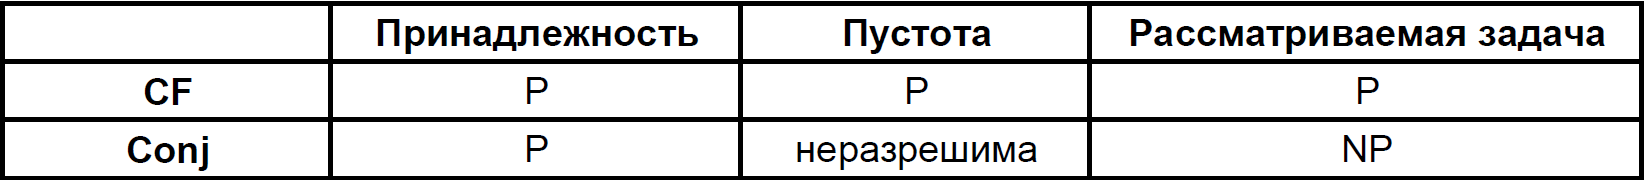
\includegraphics[width=12cm]{pictures/azimov-spbu-okhotin_tab1.png}
 \label{azimov-spbu-table}
\end{table}

\section{Связь задачи генерации строк с синтаксическим анализом графов для КС-языков}

Рассмотрим задачу синтаксического анализа графа $G = (Q, \Sigma, \delta)$ с использованием контекстно-свободной грамматики $C = (N, \Sigma, P)$ и различных семантик запроса.

\textbf{\textit{Relational} семантика запроса.} Зафиксируем нетерминал $a \in N$ и вершины графа $m, n \in Q$. При использовании данной семантики запроса необходимо проверить пустоту КС-языка $L(C,a) \cap L(G,m,n)$. Чтобы использовать для этой задачи генератор строк, необходимо построить КС-грамматику, порождающую язык $L(C,a) \cap L(G,m,n)$. В качестве такой грамматики используется аннотированная грамматика $C_{G} = (N_{G}, \Sigma, P_{G})$. А построив данную грамматику мы автоматически решаем поставленную задачу. Действительно, если $a[m,n] \notin N_{G}$, то $L(C,a) \cap L(G,m,n) = \emptyset$, а если $a[m,n] \in N_{G}$, то $L(C,a) \cap L(G,m,n) \ne \emptyset$. Поэтому нет необходимости в применении генератора строк для поиска ответа на запрос с \textit{relational} семантикой.

\textbf{\textit{All-path} семантика запроса.} Зафиксируем нетерминал $a \in N$ и вершины графа $m, n \in Q$. В данной вариации задачи синтаксического анализа графов необходимо предъявить все такие пути из вершины $m$ в вершину $n$, что метки на их ребрах образуют строку из языка $L(C,a)$. Совокупность всех строк, порождаемых такими путями, будет являться КС-языком $L(C,a) \cap L(G,m,n)$. Чтобы использовать генератор строк этого языка, необходимо построить КС-грамматику его порождающую. В качестве такой грамматики используется аннотированная грамматика $C_{G} = (N_{G}, \Sigma, P_{G})$. Причем, в работе~\cite{azimov-spbu-hellings2} эту грамматику и предлагают в качестве ответа на запрос с \textit{all-path} семантикой. Одно из преимуществ данного решения заключается в том, что имеется возможность компактно хранить бесконечное множество путей, которое может возникнуть при наличии цикла в графе $G$. Поэтому нет необходимости в применении генератора строк для поиска ответа на запрос с \textit{all-path} семантикой. Но генератор строк может быть использован для получения конкретных строк пользователем из КС-грамматики $L(C,a) \cap L(G,m,n)$. Это похоже на использование следующей (\textit{single-path}) семантики запроса, но в ней выдается один путь (и, соответственно, одна строка), когда здесь можно последовательно выдавать все новые строки из языка $L(C,a) \cap L(G,m,n)$.

Таким образом, в рассматриваемой задаче имеется возможность использовать генератор строк аннотированной КС-грамматики $C_{G}$, порождающей язык $L(C,a) \cap L(G,m,n)$. Как уже было замечено, $L(C,a) \cap L(G,m,n) \ne \emptyset \Leftrightarrow a[m,n] \in N_{G}$. Поэтому после построения аннотированной грамматики можно сразу определить пуст ли язык $L(C,a) \cap L(G,m,n)$. Необходимость применения генератора строк остается только в случае $L(C,a) \cap L(G,m,n) \ne \emptyset$. Поэтому далее считаем, что $L(C,a) \cap L(G,m,n) \ne \emptyset$, и будем исследовать возможность применения генератора строк КС-языка $L(C,a) \cap L(G,m,n)$ для последовательного предоставления отдельных строк пользователю.

Будем генерировать строку, соответствующую одному из пяти видов ограничений, представленных на рис.~\ref{azimov-spbu-tasks}. Во всех случаях имеется ограничение сверху (лексикографическое или по длине строки), что позволяет свести задачу генерации строк заданного языка к конечному числу проверок на принадлежность строк этому языку. А так как рассматриваемый лексикографический порядок в работе~\cite{azimov-spbu-Okhotin} также упорядочивает строки по длине, то во всех пяти видах ограничений мы ограничиваем генерируемую строку длиной сверху. Поэтому чтобы гарантировать генерацию строки, необходимо знать строку минимальной длины из рассматриваемой грамматики (или лексикографически наименьшую строку). Для КС-грамматик существует алгоритм, позволяющий находить строку минимальной длины, что и используется в работе~\cite{azimov-spbu-Okhotin} для генерации строк КС-языка и в работе~\cite{azimov-spbu-hellings2} в задаче синтаксического анализа графов с использованием \textit{single-path} семантики запроса. Поэтому при последовательной генерации строк мы сначала решим задачу для \textit{single-path} семантики, как и в работе~\cite{azimov-spbu-hellings2}, а после, меняя ограничения, сможем генерировать новые строки. Таким образом, каждый раз будет решаться задача для \textit{single-path} семантики, но предъявляться будет не строка наименьшей длины, а строка наименьшей длины из еще не рассмотренных строк.

\textbf{\textit{Single-path} семантика запроса.} Зафиксируем нетерминал $a \in N$ и вершины графа $m, n \in Q$. При использовании данной семантики запроса необходимо проверить пустоту КС-языка $L(C,a) \cap L(G,m,n)$ и, если он не пуст, то предъявить путь из вершины $m$ в вершину $n$, такой что метки на ребрах этого пути образуют строку из языка $L(C,a)$. В качестве такого пути в работе~\cite{azimov-spbu-hellings2} было решено использовать путь, соответствующий строке наименьшей длинны языка $L(C,a) \cap L(G,m,n)$. Как и в случае \textit{all-path} семантики запроса сначала строится аннотированная грамматика $C_{G} = (N_{G}, \Sigma, P_{G})$, и если она порождает не пустой язык, то в ней ищется строка минимальной длины, которая и будет соответствовать искомому пути в графе G.

Так как построение аннотированной грамматики и строки минимальной длины КС-языка $L(C,a) \cap L(G,m,n)$ необходимо для использования рассматриваемой генерации строк этого языка из работы~\cite{azimov-spbu-Okhotin}, то алгоритм решения задачи синтаксического анализа графов с использованием \textit{single-path} семантики запроса, предложенный в работе~\cite{azimov-spbu-hellings2}, и является примером использования генерации строки из КС-языка $L(C,a) \cap L(G,m,n)$.
\section{Связь задачи генерации строк с синтаксическим анализом графов для конъюнктивных языков}

Рассмотрим задачу синтаксического анализа графа $G = (Q, \Sigma, \delta)$ с использованием конъюнктивной грамматики $C$. Аналогично случаю КС-грамматик будем обозначать $L(C,a)$ --- язык, порождаемый конъюнктивной грамматикой $C$ со стартовым нетерминалом $a$. Гарантировать завершаемость алгоритма генерации строк из бесконечного языка можно либо умея решать задачу определения пустоты этого языка, либо заранее зная его непустоту. Первая проблема, с которой мы сталкиваемся, рассматривая конъюнктивные грамматики вместо КС-грамматик --- это неразрешимость задачи определения пустоты языка. Поэтому далее будем предполагать, что пересечение рассматриваемых языков $L(C,a) \cap L(G,m,n) \ne \emptyset$ и если это предположение неверно, то мы не можем гарантировать завершаемость алгоритмов, использующих генератор строк данного языка. Отсюда следует неразрешимость задачи синтаксического анализа с использованием конъюнктивного языка и \textit{relational} семантики запроса, о чем также упоминается в работе~\cite{azimov-spbu-hellings1}.

Мы легко можем задать конъюнктивную грамматику, порождающую пересечение языков $L(C,a) \cap L(G,m,n)$, так как в данном формализме присутствует явная операция пересечения. Так как при всех видах ограничений, рассматриваемых в работе~\cite{azimov-spbu-Okhotin}, применяется ограничение сверху длины генерируемой строки, то, не имея оценки сверху на $minlen$ --- минимальную длину строки непустого языка $L(C,a) \cap L(G,m,n)$, нельзя гарантировать нахождения хотя бы одной строки. То есть для любого ограничения на генерируемую строку, накладывающего, в частности, ограничение сверху на длину строки $(|w| \le m)$, может оказаться, что $minlen > m$ и генератор строк не сможет сгенерировать ни одной строки. Но никакой оценки сверху на $minlen$ найти не удастся, так как в противном случае за конечное число проверок принадлежности строки к конъюнктивному языку (эта задача разрешима и P-полна) можно было бы решить задачу проверки пустоты этого языка (эта задача является неразрешимой). Таким образом, для любых ограничений заранее неизвестно, есть ли хотя бы одна строка, удовлетворяющая этим ограничениям. Но если известно для какого то ограничения, что такая строка существует, то задача генерации строк для конъюнктивных грамматик и этих ограничений, согласно работе~\cite{azimov-spbu-Okhotin}, NP-полна.

Предположим, что найдется хотя бы одна строка, удовлетворяющая рассматриваемым ограничениям. Тогда при использовании \textit{all-path} семантики запроса, применяя алгоритм генерации строки, происходил бы просто перебор всех возможных строк и проверка на принадлежность этих строк к языку $L(C,a) \cap L(G,m,n)$, что не соответствует практическому смыслу задачи. Для задачи синтаксического анализа графов с использованием \textit{single-path} семантики запроса есть возможность сгенерировать некоторую строку непустого языка $L(C,a) \cap L(G,m,n)$ (в работе~\cite{azimov-spbu-hellings2} подчеркнута логичность выбора строки минимальной длины, но это необязательно).

\section{Заключение}

В данной работе была показана связь между задачей генерации строк, рассмотренной в работе~\cite{azimov-spbu-Okhotin}, и некоторыми вариациями задачи синтаксического анализа графов, предложенных в работе~\cite{azimov-spbu-hellings1, azimov-spbu-hellings2} и использующих контекстно-свободные и конъюнктивные грамматики.

Использование конъюнктивных языков в задачах синтаксического анализа графов мало изучено. Полученные результаты могут быть использованы в дальнейших исследованиях данной области.

\setmonofont[Mapping=tex-text]{CMU Typewriter Text}
\bibliographystyle{ugost2008ls}
\bibliography{azimov-spbu-biblio.bib}
\end{document}
